%
% Erhaltungssätze
%
\section{Erhaltungssätze
\label{buch:gauss:section:erhaltungssatz}}
\kopfrechts{Erhaltungssätze}
Das Oberflächenintegral einer 2-Form berechnet den Fluss von Materie,
Energie oder anderen physikalischen Grössen durch die Oberfläche.
Ein Erhaltungssatz beschreibt, ob und wie der Fluss die im umschlossenen
Volumen enthaltene Menge verändert.
Der Satz von Gauss stellt den Zusammenhang her zwischen Inhalt und Fluss
über das ganze Volumen und seine Oberfläche und der, die beschreibt,
was in der unmittelbaren Umgebung jedes Punktes geschieht.
Das Resultat ist die Kontinuitätsgleichung, die in diesem Abschnitt
hergeleitet und angewendet werden soll.

%
% Kontinuitätsgleichung
%
\subsection{Kontinuitätsgleichung
\label{buch:zusammenhang:erhaltungssatz:subsection:kontinuitaetsgleichung}}
%
% fig-kont.tex
%
% (c) 2025 Prof Dr Andreas Müller
%
\begin{figure}
\centering
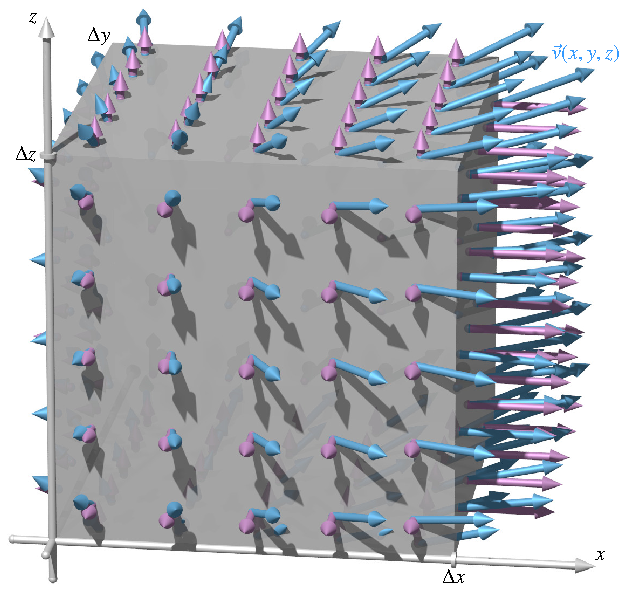
\includegraphics{chapters/050-gauss/images/kont.pdf}
\caption{Fluss des blauen Vektorfeldes durch einen Quader.
Nur die auf der Oberfläche senkrechte, violette Komponente trägt
zum Fluss bei.
\label{buch:gauss:fig:kont}}
\end{figure}
%
Wir betrachten das Vektorfeld $\vec{v}(x,y,z)$ im $\mathbb{R}^3$.
Es beschreibt die Geschwindigkeit eines Fluids der Dichte $\varrho(x,y,z)$.

Wir berechnen den Fluss des Fluids durch die Oberfläche eines Quaders
mit den Seiten $\Delta x$, $\Delta y$ und $\Delta z$.
Der Strom des Fluids ist
$\vec{\jmath}(x,y,z,t)=\varrho(x,y,z,t)\,\vec{v}(x,y,z,t)$.
Die 2-Form für den Fluss ist
\[
\omega
=
\varrho
j_x
\,dy\wedge dz
+
j_y
\,dx\wedge dz
-
j_z
\,dx\wedge dy.
\]
Der Fluss ist das Integral von $\omega$ über die Oberfläche des
Quaders.
Wir nehmen an, dass $\Delta x$, $\Delta y$ und $\Delta z$ klein
sind, so dass es gerechtfertigt ist, die Komponenten von $v$ auf
den Seitenflächen des Quaders als konstant anzusehen.
Dann ist der Fluss näherungsweise
\begin{align*}
\int_{\text{Quader}}\omega
&\approx
\Delta x\,\Delta y\,(j_z(x, y, z+\Delta z) - j_z(x, y, z))
+
\Delta x\,\Delta z\,(j_y(x, y+\Delta y, z) - j_y(x, y, z))
\\
&
\qquad
+
\Delta y\,\Delta z\,(j_x(x+\Delta x, y, z) - j_x(x, y, z))
\intertext{Gehen die Seitenlängen gegen $0$, geht auch das Integral
gegen 0.
Teilt man durch das Volumen $V=\Delta x\,\Delta y\,\Delta z$, bleibt}
\frac{1}{V}\int_{\text{Quader}} \omega
&=
\frac{j_z(x, y, z+\Delta z) - j_z(x, y, z)}{\Delta x}
+
\frac{j_y(x, y+\Delta y, z) - j_y(x, y, z)}{\Delta y}
\\
&\qquad
+
\frac{j_x(x+\Delta x, y, z) - j_x(x, y, z)}{\Delta z}
\intertext{Der Grenzwert für $\Delta x\to 0$, $\Delta y\to 0$ und
$\Delta z\to 0$ wird}
&\to
\frac{\partial j_z}{\partial z}
+
\frac{\partial j_y}{\partial y}
+
\frac{\partial j_x}{\partial x}
=
\operatorname{div}\vec{\jmath}(x,y,z).
\end{align*}
Die Divergenz misst also den Fluss durch einen infinitesimalen 
Quader.

Der Fluss beschreibt auch, mit welcher Geschwindigkeit sich die Menge
des Materials im Quader ändert.
Dies kann jedoch berechnet werden, indem die Masse zu verschiedenen
Zeiten berechnet wird.
Mit der Dichte $\varrho(x,y,z,t)$ des Fluids ist die Änderung der 
Masse gegeben durch
\begin{align*}
\Delta m
&=
\int_{\text{Quader}} \varrho(x,y,z,t+\Delta t)\,dx\,dy\,dz
-
\int_{\text{Quader}} \varrho(x,y,z,t)\,dx\,dy\,dz.
\intertext{Für einen kleinen Quader kann man wieder annehmen, dass die
Dichte im Quader im Wesentlichen konstant ist, der Masseunterschied
lässt sich daher als}
\Delta m
&\approx
(\varrho(x,y,z,t+\Delta t)
-
\varrho(x,y,z,t))
\,\Delta x\,\Delta y\,\Delta z.
\end{align*}
Die zeitliche Änderung der Dichte ist
\begin{align*}
\frac{\Delta m}{\Delta x\,\Delta y\,\Delta z\,\Delta t}
&=
\frac{\varrho(x,y,z,t+\Delta t)-\varrho(x,y,z,t)}{\Delta t}
\end{align*}
Der Grenzwert $\Delta t\to 0$ ergibt die Zeitableitung von $\varrho$
und damit die Gleichung
\begin{equation}
\frac{\partial \varrho}{\partial t}
=
\operatorname{div}\vec{\jmath}
=
\operatorname{div}(\varrho\vec{v}).
\label{buch:gauss:erhaltungssatz:eqn:kontinuitaet}
\end{equation}
Dies ist die {\em Kontinuitätsgleichung}.

%
% Anwendungen
%
\subsection{Anwendungen}
Die Kontinuitätsgleichung tritt in vielfältiger Form in den verschiedensten
Gebieten auf.

%
% Wärmeleitung
%
\subsubsection{Wärmeleitung}
Wir betrachten die Verteilung von Wärmeenergie in einem Festkörper.
Die Energiedichte $\varrho$ kann aus der orts- und zeitabhängigen
Temperatur $T(x,y,z,t)$ und der spezifischen Wärme $c$ des Materials
durch $\varrho = cT$ berechnet werden.

Der Wärmefluss in Richtung des Vektors $\vec{v}$ ist proportional
zur Temperaturdifferenz in diese Richtung:
\[
\frac{d}{ds}
T(x+s\vec{v},t)\bigg|_{s=0}
=
D_{\vec{v}} T.
\]
Die Richtungsableitung kann durch das Differential von $T$
ausgedrückt werden.
Die Koeffizienten von $dT$ sind die partiellen Ableitungen
\[
dT
=
\frac{\partial T}{\partial x}\,dx
+
\frac{\partial T}{\partial y}\,dy
+
\frac{\partial T}{\partial z}\,dz
\]
Der Proportionalitätsfaktor ist die Wärmeleitfähigkeit $\kappa$.
Damit wird der Wärmestrom:
\[
j_x\,dx
+
j_y\,dy
+
j_z\,dz
=
\kappa
dT
\qquad\text{oder}\qquad
\vec{\jmath}
=
\kappa
\operatorname{grad} T
\]
in vektorieller Schreibweise.
Die Erhaltung der Energie wird durch die Kontinuitätsgleichung
für die Energiedichte $\varrho$ und den Stromvektor $\vec{\jmath}$
ausgedrückt.
Durch die Temperatur ausgedrückt besagt sie
\[
\frac{\partial }{\partial t}
(cT)
=
\operatorname{div}(\kappa\operatorname{grad}T).
\]

In einem homogenen Medium darf man annehmen, dass $c$ und $\kappa$ konstant
sind.
Die Kontinuitätsgleichung wird damit zu
\begin{align*}
c\frac{\partial T}{\partial t}
&=
\kappa
\operatorname{div}\operatorname{grad}T
\\
&=
c
\biggl(
\frac{\partial}{\partial x}
\frac{\partial T}{\partial x}
+
\frac{\partial}{\partial y}
\frac{\partial T}{\partial y}
+
\frac{\partial}{\partial z}
\frac{\partial T}{\partial z}
\biggr)
\\
&=
\kappa
\biggl(
\frac{\partial^2 T}{\partial x^2}
+
\frac{\partial^2 T}{\partial y^2}
+
\frac{\partial^2 T}{\partial z^2}
\biggr)
=
\kappa \Delta T
\end{align*}
mit dem Laplace-Operator $\Delta$.

%
% Elektrische Ladung
%
\subsubsection{Elektrische Ladung}
Die elektrische Ladung ist erhalten.
Die elektrische Stromdichte $\vec{\jmath}$ ist der Vektor, der die Ladung
angibt, die in einer Zeiteinheit durch eine Flächeneinheit quer zur
Stromrichtung angibt.
Für die Ladungsdichte $\varrho$ und die Stromdichte $\vec{\jmath}$
muss daher die Kontinuitätsgleichung
\[
\frac{\partial\varrho}{\partial t}
=
\operatorname{div} \vec{\jmath}
\]
gelten.

%
% Erhaltungssätze für Vierervektoren
%
\subsubsection{Erhaltungssätze für Vierervektoren}
In der speziellen Relativitätstheorie wird gelehrt, dass Raum- und
Zeitkoordinaten nicht separat behandelt werden sollten, sondern als
Komponenten eines Raum-Zeit-Kontinuums.
Eine Lorentz-Transformation kann Orts- und Zeitkoordinaten  ``vermischen''
was zu den Phänomen der Zeitdilatation und der Raumkontraktion führt.
Es beutet, dass zu vektoriellen Grössen, mit denen man in der newtonschen
Mechanik rechnet, jeweils auch eine Zeit-Komponenten gefunden werden
muss.
Zusammen bilden diese Komponenten einen Vierervektor, der die gleichen
Transformationsregeln befolgt, wie Ort und Zeit.
Das Skalarprodukt solcher Vierervektoren mit sich selbst bleibt
bei Lorentz-Transformationen erhalten.
Das Skalarprodukt eines Viervektors $x^k$ in der speziellen
Relativitätstheorie ist
\[
(x^0)^2
-
(x^1)^2
-
(x^2)^2
-
(x^3)^2,
\]
welches auch durch den metrischen Tensor
\[
(g_{ik})
=
\begin{pmatrix}
1&0&0&0\\
0&-1&0&0\\
0&0&-1&0\\
0&0&0&-1
\end{pmatrix}
\]
beschrieben werden kann.

Für den elektrischen Strom mit den Komponenten $j_1,j_2,j_3$ ist die
zugehörige Zeitkomponenten die Ladungsdichte, wir sind also gezwungen
$j_0=\varrho$ zu schreiben.
Die Kontinuitätsgleichung
\begin{align*}
\frac{\partial\varrho}{\partial t}
&=
\frac{\partial j_1}{\partial x^1}
+
\frac{\partial j_2}{\partial x^2}
+
\frac{\partial j_3}{\partial x^3}
\intertext{bekommt dann die Form}
\frac{\partial j_0}{\partial x^0}
&-
\frac{\partial j_1}{\partial x^1}
-
\frac{\partial j_2}{\partial x^2}
-
\frac{\partial j_3}{\partial x^3}
=
0.
\end{align*}
Dies kann etwas kompakter auch als
\[
\sum_{i,k=0}^3
g^{ik}\frac{\partial}{\partial x^k}j_i
=
0
\]
geschrieben werden kann.
Dies deutet an, dass es einen Differentialoperator, die Viererdivergenz,
gibt, der die Ladungserhaltung beschreiben kann.
Die genaue Definition wird in Kapitel~\ref{chapter:hodge} mit Hilfe des
Hodge-Operators gegeben.


